\section{Monday for MAT3006}\index{Monday_lecture}
Our first quiz will be held on this Wednesday.

\paragraph{Reviewing}
We have shown that 
the algebra $\mathcal{A}\subseteq\mathcal{C}(X)$ with separation, non-vanishing property 
implies $\overline{\mathcal{A}} = \mathcal{C}(X)$.

Now we show that if $\overline{\mathcal{A}} = \mathcal{C}(X)$, then the algebra $\mathcal{A}$ has separation, non-vanishing property:
\begin{enumerate}
\item
Suppose on the contrary that $\mathcal{A}$ is not separating, i.e., 
there exists $x_1,x_2\in X$ such that $\phi(x_1)=\phi(x_2)$, $\forall\phi\in\mathcal{A}$.

By the defintion of closure, it's clear that for given $S\subseteq(X,d)$, $\forall x\in\overline{S}$, there exists a sequence $\{S_n\}$ in $S$ such that $S_n\to x$.

Construct $f\in\mathcal{C}(X)$ defined by $f(x) = d(x,x_1)$. It follows that
\[
\begin{array}{ll}
f(x_1)=0,
&
f(x_2) = d(x_2,x_1):=k>0
\end{array}
\]
Now we claim that $f\notin\overline{\mathcal{A}}$, since otherwise there exists $\{\phi_n\}$ in $\mathcal{A}$ such that $\phi_n\to f$, i.e.,
\[
\begin{array}{lll}
\phi_n(x_1)\to f(x_1),
&
\phi_n(x_2)\to f(x_2),
&
\phi_n(x_1)=\phi_n(x_2),\forall n,
\end{array}
\]
i.e., $0=f(x_1)=f(x_2)>0$.
\item
Suppose on the contrary that $\mathcal{A}$ is not non-vanishing, i.e., there exists some $x_0\in X$ such that $\phi(x_0)=0,\forall \phi\in\mathcal{A}$. Construct $g\in\mathcal{C}(X)$ defined by $g(x) = d(x,x_0)+1$. 

Following the similar idea, we can show that there does not exist $\phi_n\in\mathcal{A}$ such that $\phi_n\to g$, i.e., $g\notin\overline{\mathcal{A}}$, which is a contradiction.
\end{enumerate}


\begin{example}
\begin{enumerate}
\item
Let $X\subseteq\mathbb{R}^n$ be a compact space. 
Then the polynomial ring 
\[
\mathbb{R}[x_1,\dots,x_n]=\{\text{Polynomials in $n$ variables with coefficients in $\mathbb{R}$}\}
\]
 forms a dense set in $\mathcal{C}(X)$.

It's clear that the set $\mathbb{R}[x_1,\dots,x_n]$ satisfies the separating and non-vanishing property. For the special case $n=1$ and $X=[a,b]$, we get the Weierstrass Approximation Theorem.
\item
In particular, when $X=S^1\subseteq\mathbb{R}^2$, we imply 
$\mathbb{R}[x,y]$ is dense in $\mathcal{C}(S^1)$.
\end{enumerate}
\end{example}
\subsection{Stone-Weierstrass Theorem in $\mathbb{C}$}

Consider the circle $S^1\subseteq\mathbb{C}$ and the mappings
\[
\begin{array}{ll}
&c:S^1\to\mathbb{R}\\
\text{with}&e^{i\theta}\to\cos\theta
\end{array}\qquad
\begin{array}{ll}
&s:S^1\to\mathbb{R}\\
\text{with}&e^{i\theta}\to\sin\theta
\end{array}
\]
are both continuous.

The algebra formed by $s$ and $c$ is given by
\[
\mathcal{J}:=\inp{c}{s}=\Span\{\cos^m\theta \sin^n\theta\mid m,n\in\mathbb{N}\}
\]
\begin{enumerate}
\item
The $\mathcal{J}$ satisfies both separating and non-vanishing property, which implies $\overline{\mathcal{J}} = \mathcal{C}(S^1)$.
\item
Suppose $f:\mathbb{R}\to\mathbb{R}$ is a continuous, $2\pi$-periodic mapping. It's easy to construct a continuous mapping $\tilde f:S^1\to\mathbb{R}$ such that the diagram below commutes:
\begin{figure}[H]
\centering
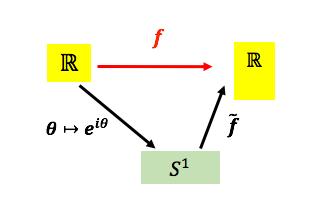
\includegraphics[width=0.5\textwidth]{week5/p_2}
\end{figure}
Or equivalently, $f(\theta) = \tilde{f}(e^{i\theta})$ for some $\tilde{f}\in\mathcal{C}(S^1)$.
Since $\overline{\mathcal{J}} = \mathcal{C}(S^1)$, we can approximate $\tilde{f}\in\mathcal{C}(S^1)$ by $\inp{\cos\theta}{\sin\theta}$, which implies that the $f(\theta)$ can be approximated by
\[
\sum_{m,n\in\mathbb{N}}a_{m,n}\cos^m\theta\sin^n\theta.
\]
Since $\Span\{\cos^m\theta\sin^n\theta\}_{m,n\in\mathbb{N}} = \Span\{\cos(m\theta),\sin(n\theta),1\}_{m,n\in\mathbb{N}}$, we imply $f(\theta)$ can be approximated by
\[
\sum_{m,n\in\mathbb{N}}a_m\cos(m\theta)+b_n\sin(n\theta).
\]
Or equivalently, for any $\varepsilon>0$, there exists $N>0$ and $a_m,a_n\in\mathbb{R}$ such that 
\begin{equation}\label{Eq:5:1}
\left|f(\theta) - 
\left(
a_0+\sum_{m=1}^Na_m\cos(m\theta) + \sum_{n=1}^Nb_n\sin(n\theta)
\right)
\right|<\varepsilon,\quad
\forall\theta\in[0,2\pi].
\end{equation}
\end{enumerate}
\begin{remark}
The natural question is that do we have the following equation hold:
\begin{equation}\label{Eq:5:2}
f(\theta) = a_0 + \sum_{m=1}^\infty a_m\cos(m\theta) + \sum_{n=1}^\infty b_n\sin(n\theta)
\end{equation}
It seems that Eq.(\ref{Eq:5:2}) above is equivalent to the expression in (\ref{Eq:5:1}). However, unlike the Taylor expansion, the values of $a_m,a_n,M,N$ may change once we switch the number $\varepsilon>0$. 

Therefore, Eq.(\ref{Eq:5:2}) does not hold for most functions, but only for some functions with nice structure.
\end{remark}


\paragraph{Fourier Analysis}
Given the condition that the Eq.(\ref{Eq:5:2}) holds. How can we get the values of $a_m$ and $b_n$? The way is to take ``inner product'' between $f(\theta)$ and trigonometric functions. For example, by taking the inner product with $\cos(k\theta)$ for Eq.(\ref{Eq:5:2}) both sides, we have
\begin{align*}
\int_{-\pi}^\pi f(\theta) \cos(k\theta)\diff\theta &= \frac{a_0}{2}\int_{-\pi}^\pi\cos(k\theta)\diff\theta\\&
+
\sum_{m=1}^\infty a_m\int_{-\pi}^\pi\cos(m\theta)\cos(k\theta)\diff\theta
+
\sum_{m=1}^\infty b_n\int_{-\pi}^\pi\sin(n\theta)\cos(k\theta)\diff\theta\\
&=\pi\cdot a_k
\end{align*}
Following the same trick, we obtain:
\begin{equation}\label{Eq:5:3}
\begin{aligned}
a_k&=\frac{1}{\pi}\int_{-\pi}^\pi f(\theta)\cos(k\theta)\diff\theta\\
b_k&=\frac{1}{\pi}\int_{-\pi}^\pi f(\theta)\sin(k\theta)\diff\theta
\end{aligned}
\end{equation}

Naturally, we define the fourier expansion for general $f(\theta)$, even though we don't verify whether (\ref{Eq:5:2}) holds or not:
\[
g_N(\theta) = \frac{a_0}{2}+\sum_{n=1}^Na_m\cos(m\theta)+\sum_{n=1}^Nb_n\sin(n\theta),
\]
where the term $a_m$ and $b_n$ follow the definition in (\ref{Eq:5:3}).
The natural question is that whether $g_N(\theta)\to f(\theta)$ as $N\to\infty$?

\subsection{Baire Category Theorem}
\paragraph{Motivation}
The set $\mathcal{P}[a,b]\subseteq\mathcal{C}[a,b]$ is dense by Weierstrass Approximation.
However, it is not ``abundant'' in $\mathcal{C}[a,b]$, just like $\mathbb{Q}\subseteq\mathbb{R}$ is dense in $\mathbb{R}$.
(Every $r\in\mathbb{R}$ is a limit of a sequence in $\mathbb{Q}$)

The set $\mathbb{Q}$ is countable yet $\mathbb{R}\setminus\mathbb{Q}$ is uncountable, i.e., there are many more holes in $\mathbb{R}\setminus\mathbb{Q}$.

\begin{definition}[Nowhere Dense]
A subset $S\subseteq(X,d)$ is \emph{nowhere dense} if $\overline{S}$ does not contain any open ball, i.e., 
\[
\text{$X\setminus\overline{S}$ is dense in $X$}
\]
\end{definition}
For example, a single point is nowhere dense.

\begin{theorem}
Let $\{E_i\}_{i=1}^\infty$ be a collection of nowhere dense sets in a complete metric space $(X,d)$. 
Then the set
\[
\bigcup_{i=1}^\infty \overline{E_i}
\]
also does not contain any open ball.
\end{theorem}
\begin{proof}
I have no time to review and modify the proof during the lecture. Therefore, we encourage the reader to go through the proof in the note
\begin{quotation}
W,Ni \& J. Wang (January, 2019). Lecture Notes for MAT2006. Retrieved from 
\url{https://walterbabyrudin.github.io/information/information.html}
\end{quotation}
Of course, I will also add the proof in this note during this week.
%
%Assume that all $E_i$ are closed, i.e., $E_i=\overline{E_i}$. We want to show that for any ball $B$,
%\[
%B\cap\left(\bigcup_{i=1}^\infty E_i\right)^c\ne\emptyset
%\]
%Since $B\cap E_1^c$ is open, non-empty (because $E_1$ is nowhere dense), we pick $B_1\subseteq B$ such that 
%\begin{enumerate}
%\item
%$B_1\subseteq B\cap E_1^c$, radius$(B_1)\le\frac{1}{2}$radius(B)
%\item
%$\overline{B}_1\cap E_1=\emptyset$
%\end{enumerate}
%Continue the argument for $B_1$ on $E_2^c$: we pick $B_2\subseteq B_1$ such that
%\begin{enumerate}
%\item
%$B_2\subseteq B_1\cap E_2^c$ and radius$(B_2)\le\frac{1}{2}$radius($B_1$)
%\item
%$\overline{B}_2\cap E_2=\emptyset$
%\end{enumerate}
%We continue to get a sequence of balls $\{B_n\}$ such that
%\begin{enumerate}
%\item
%$\overline{B}_{i+1}\subseteq B_i,\ \forall i$
%\item(*)
%$\overline{B}_{i+1}\subseteq\cup_{k=1}^{i+1}E_i$
%\item
%radius of $B_n$ reduces by half
%\end{enumerate}
%Therefore, consider $x_n=\text{center}(B_n)$, we imply $\{x_n\}$ is Cauchy. 
%
%By completeness, $x\to x_\infty\in X$. We claim that $x_\infty\notin E_i,\forall i$. 
%Suppose on the contrary that $x_\infty\in E_N$ for some $N$. Then
%\[
%x_\infty\in\overline{B}_N,\forall n=1,2,\dots
%\]
%which implies $x_\infty\in B_N$, which contradicts to the fact (*).
\end{proof}

































